
\section{Modelagem do robô}

Um veículo omnidirecional de 3 rodas no contexto deste trabalho é um robô
holonômico capaz de se mover em translação e rotação simultaneamente e
independentemente \cite{mobile_manipulator_robot}. Sua geometria básica se 
baseia em rodas equidistantes em uma circunferência, com 120° de separação entre
 si, tangenciando o perímetro do chassi do veículo, como demonstrado na figura
 1.

\begin{figure}[ht]
	\centering
	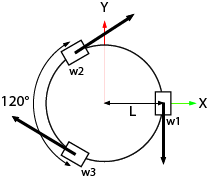
\includegraphics{figures/model}
	\caption{Diagrama do modelo matemático do robô}
\end{figure}

Robôs omnidirecionais tais como esse são particularmente úteis porque permitem
 maior manobrabilidade e eficiência, a um custo de maior complexidade na sua
 construção e controle. \cite{dynamical_models_for_omni_directional_robots}

\subsection{Modelagem Cinemática - Dedução da matriz por cinemática direta}

$\overrightarrow{V}$ é o vetor de velocidade linear do robô, $V_{w1}$, $V_{w2}$,
$V_{w3}$ são as velocidades lineares das rodas 1,2,3. 
$\omega $ é a velocidade angular do robô a partir do seu centro geométrico.
$L$ é a distância entre o centro de geométrico da roda e o centro de geométrico
do robô.


\begin{figure}[ht]
	\centering
	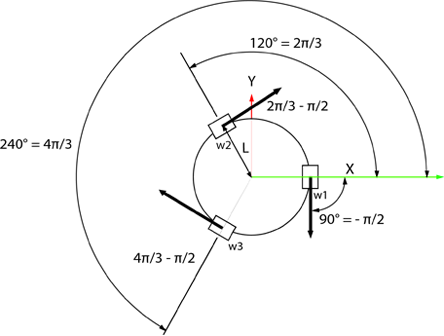
\includegraphics[width=0.8\textwidth]{figures/digram_model_dedution}
	\caption{Diagrama do modelo matemático do robô, com valores dos ângulos das
	rodas}
\end{figure}

\begin{equation}
    \begin{split}
        \overrightarrow{V}_{l} = 
        \overrightarrow{V}_{w1}
        + \overrightarrow{V}_{w2}
        + \overrightarrow{V}_{w3}
    \end{split}
\end{equation}

\begin{equation}
    \begin{split}
        \overrightarrow{\omega} = 
        \frac{\vert\overrightarrow{V}_{w1}\vert}{L}
        + \frac{\vert\overrightarrow{V}_{w2}\vert}{L}
        + \frac{\vert\overrightarrow{V}_{w3}\vert}{L}
    \end{split}
\end{equation}


\begin{gather*}
        V_{l} \angle \theta =  
        V_{w1} \angle \left(-\frac{\pi}{2}\right) 
        + V_{w2} \angle \left(\frac{2\pi}{3}-\frac{\pi}{2}\right) 
        + V_{w3} \angle \left(\frac{4\pi}{3}-\frac{\pi}{2}\right) 
\end{gather*}

\begin{align*}
    V_{l} \cos{ \theta } + jV_{l} \sin{\theta} =  
    V_{w1} \cos{ \left(-\frac{\pi}{2}\right)} + jV_{w1} \sin{ \left(-\frac{\pi}{2}\right) } \\
    + V_{w2}  \cos{ \left(\frac{\pi}{6}\right) } + jV_{w2}  \sin{ \left(\frac{\pi}{6}\right) }  \\
    + V_{w3} \cos{ \left(\frac{5\pi}{6}\right) } + jV_{w3}  \sin{ \left(\frac{5\pi}{6}\right) } 
\end{align*}

\begin{equation*}
    \begin{split}
        \omega = 
        \frac{V_{w1}}{L}
        + \frac{V_{w2}}{L}
        + \frac{V_{w3}}{L}
    \end{split}
\end{equation*}


\begin{gather}
	\begin{bmatrix} V\cdot \cos{\theta} \\  V\cdot \sin{\theta} \\  \omega \end{bmatrix}
	=
	\begin{bmatrix}
		\cos{\left(-\frac{\pi}{2}\right)} & \cos{\left(\frac{\pi}{6}\right)} & \cos{\left(\frac{5\pi}{6}\right)} \\
		\sin{\left(-\frac{\pi}{2}\right)} & \sin{\left(\frac{\pi}{6}\right)} & \sin{\left(\frac{5\pi}{6}\right)} \\
		\frac{1}{L} & \frac{1}{L} & \frac{1}{L}
	\end{bmatrix}
	\cdot
	\begin{bmatrix} V_{w1} \\  V_{w2} \\  V_{w3} \end{bmatrix}
\end{gather}



Matriz da cinemática direta:

\begin{gather}
	\begin{bmatrix}
		\cos{\left(-\frac{\pi}{2}\right)} & \cos{\left(\frac{\pi}{6}\right)} & \cos{\left(\frac{5\pi}{6}\right)} \\
		\sin{\left(-\frac{\pi}{2}\right)} & \sin{\left(\frac{\pi}{6}\right)} & \sin{\left(\frac{5\pi}{6}\right)} \\
		\frac{1}{L} & \frac{1}{L} & \frac{1}{L}
	\end{bmatrix}
	=
	\begin{bmatrix}
		0 & \sqrt{3}/2 & -\sqrt{3}/2 \\
		-1 & 1/2 & 1/2  \\
		1/L & 1/L & 1/L
	\end{bmatrix}
\end{gather}



Matriz inversa:


\begin{gather}
	\begin{bmatrix} V_{w1} \\  V_{w2} \\  V_{w3} \end{bmatrix}
	=
	\begin{bmatrix}
		0 & -2/3 & L/3 \\
		1/\sqrt{3} & 1/3 & L/3\\
		-1/\sqrt{3} & 1/3 & L/3
	\end{bmatrix}
	\cdot
	\begin{bmatrix} V\cdot \cos{\theta} \\  V\cdot \sin{\theta} \\  \omega \end{bmatrix}
\end{gather}


A matriz 3.5 é a matriz de cinemática do robô.
As entradas são o vetor velocidade linear e a velocidade angular do robô, e as
saídas são as velocidades lineares de cada uma das rodas.

Desconsiderando a velocidade angular, é possível observar os vetores velocidades
das rodas e o vetor velocidade linear do robô na figura \ref{simulacao}, que
foi gerada por meio de simulação em Python. O código fonte da simuação pode ser encontrada no projeto
\url{https://github.com/dcarve/tg-robot/tree/master/simulation/vectors_simulation/src}

\begin{figure}[ht]
	\centering
	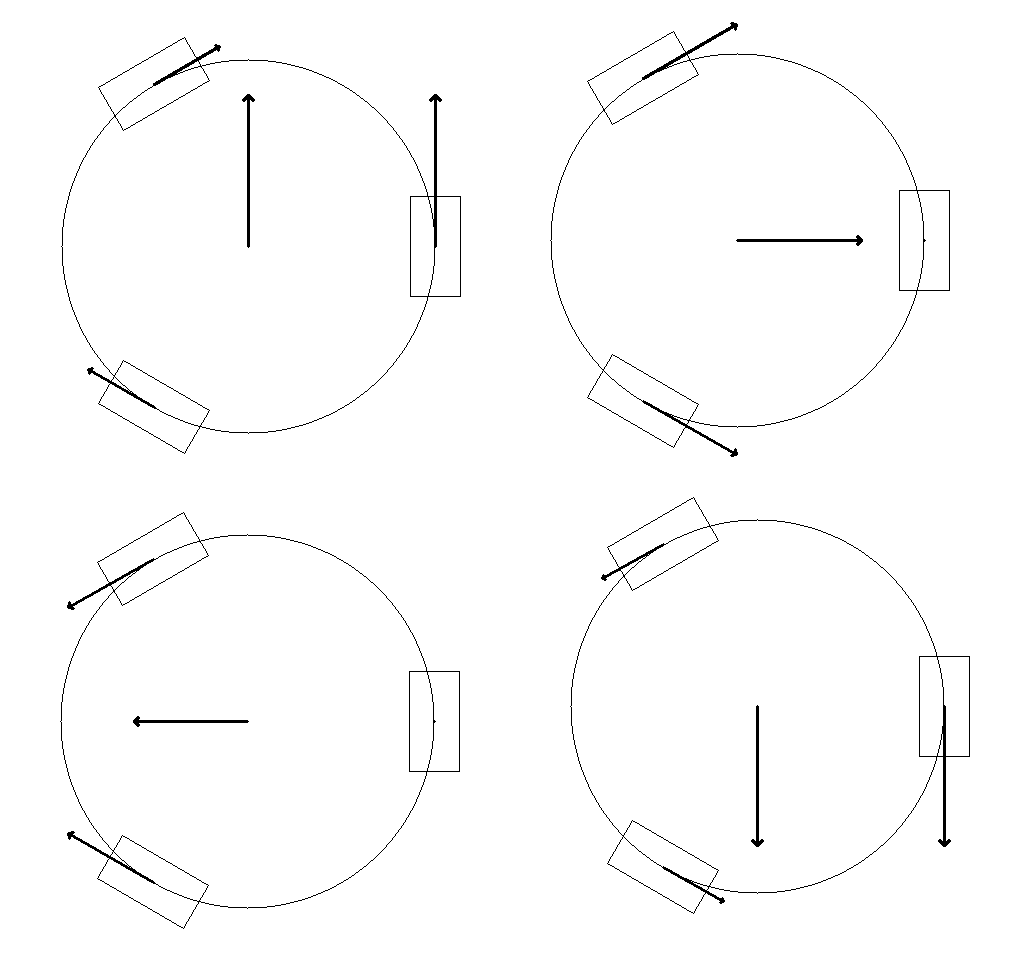
\includegraphics[width=0.7\textwidth]{figures/simulacao}
	\caption{Simulação dos vetores}
	\label{simulacao}
\end{figure}

